% 内积空间：正交与投影（正交补、标准正交基、Gram--Schmidt正交化与QR分解、正交投影）。

\section{正交与投影}
\label{sec:ls-orthogonality-and-projection}

内积给出了两个向量之间的正交关系。本节把它推广到向量与子空间之间，把向量分解为子空间中的分量与和子空间正交的剩余部分。接着引入标准正交基，并用Gram--Schmidt正交化构造它；最后用标准正交基写出正交投影，证明它给出唯一的最近点。

\subsection{正交补与正交分解}
\label{sec:ls-orthogonality}

Gram矩阵记录的是一组向量两两之间是否正交。本小节考虑一个向量与整个子空间的正交，由此得到一个由内积唯一确定的补空间，并用它证明四个基本子空间之间的垂直关系。

\paragraph{正交补}
第~\ref{sec:ls-direct-sum}节说明，一个子空间的补空间一般不唯一。有了内积，可以挑出一个由垂直关系确定的补空间。设$U$是有限维内积空间$V$的子空间，与$U$中每个向量都正交的向量组成集合
\[
 U^\perp=\{\bm r\in V:\langle\bm u,\bm r\rangle=0,\ \forall\bm u\in U\},
\]
称为$U$的\term{正交补}（orthogonal complement）。由内积的双线性，$U^\perp$对线性组合封闭，是子空间。要检查$\bm r\in U^\perp$，只需检查它与$U$的一组基逐个正交，因为与基向量都正交的向量，也与基向量的每个组合正交。

\paragraph{正交直和}
下面证明正交补确实是一个补空间，而且分解可以由Gram矩阵算出。
\begin{lemma}[正交直和]
\label{lem:ls-orthogonal-decomposition}
设$U$是有限维内积空间$V$的子空间，则每个$\bm x\in V$唯一分解为$\bm x=\bm u+\bm r$，其中$\bm u\in U$、$\bm r\in U^\perp$；即$V=U\oplus U^\perp$。
\end{lemma}
\begin{proof}
取$U$的一组基$\bm b_1,\ldots,\bm b_r$。它线性无关，所以Gram矩阵$\bm G$正定，从而可逆。对任意$\bm x$，令$\bm u=\sum_j a_j\bm b_j$，并要求$\bm r=\bm x-\bm u$与每个$\bm b_i$正交，得到系数方程
\[
 \sum_j g_{i,j}a_j=\langle\bm b_i,\bm x\rangle\qquad(i=1,\ldots,r),
\]
写成矩阵形式就是Gram方程
\begin{equation}
 \bm G\bm a=(\langle\bm b_i,\bm x\rangle)_i .
 \label{eq:ls-gram-equation}
\end{equation}
$\bm G$可逆，所以系数唯一解出；残差$\bm r$与全部基向量正交，因而落在$U^\perp$。

若$\bm x=\bm u+\bm r=\bm u'+\bm r'$是两种分解，则$\bm u-\bm u'=\bm r'-\bm r$同时属于$U$与$U^\perp$。它与自身正交，长度为零，故两种分解相同。
\end{proof}
所以正交补是$U$的一个补空间，并且由内积唯一确定；$V=U\oplus U^\perp$称为正交直和。由维数公式，$\dim U^\perp=\dim V-\dim U$。下面在$\mathbb R^3$中做一次分解。
\begin{example}[向一条直线的正交分解]
\label{ex:ls-orthogonal-decomposition-line}
在$\mathbb R^3$中取欧氏内积，把$\bm y=(1,1.1,0.9)^\top$分解到直线$U=\operatorname{span}\{\bm c_1\}$及其正交补上，其中$\bm c_1=(1,1,1)^\top$。与$\bm c_1$正交就是坐标和为零，所以$U^\perp$是坐标和为零的平面。

$U$只有一个基向量，Gram方程只有一个未知数：
\[
 \langle\bm c_1,\bm c_1\rangle a=\langle\bm c_1,\bm y\rangle,\qquad\text{即}\ 3a=3,
\]
所以$a=1$。于是
\[
 \begin{gathered}
 \bm u=\bm c_1=(1,1,1)^\top,
 \\
 \bm r=\bm y-\bm u=(0,0.1,-0.1)^\top,
 \end{gathered}
\]
$\bm r$的坐标和为零，确实属于$U^\perp$。

所以$\bm y=\bm u+\bm r$就是$\bm y$在正交直和$\mathbb R^3=U\oplus U^\perp$中的分解：沿$\bm c_1$方向的部分是三个坐标的公共水平$1$，剩下的$(0,0.1,-0.1)^\top$记录各坐标偏离这个水平的程度。
\end{example}
这里只得到了正交分量的存在与唯一。它为什么是$U$中离$\bm y$最近的点，将在第~\ref{sec:ls-orthogonal-projection}节用标准正交基证明。

取两次正交补会回到原来的子空间：$(U^\perp)^\perp=U$。一方面，$U$中每个向量与$U^\perp$中每个向量正交，所以$U\subseteq(U^\perp)^\perp$。另一方面，对$U^\perp$用上面的维数关系，
\[
 \dim(U^\perp)^\perp=\dim V-\dim U^\perp=\dim U .
\]
二者包含且同维，由第~\ref{sec:ls-dimension}节，两者相等。

\paragraph{四个基本子空间的正交关系}
示例~\ref{ex:ls-rank-one-four-subspaces}显示，行空间的方向与零空间垂直，列空间的方向与左零空间垂直。现在在$\mathbb R^d$与$\mathbb R^m$上取欧氏内积，证明这对任何矩阵都成立。
\begin{theorem}[四个基本子空间的正交关系]
\label{thm:ls-four-subspaces-orthogonality}
设$\bm A\in\mathbb R^{m\times d}$，$\mathbb R^d$与$\mathbb R^m$取欧氏内积。则
\begin{equation}
\begin{gathered}
\operatorname{null}(\bm A)=\operatorname{range}(\bm A^\top)^\perp,\\
\operatorname{null}(\bm A^\top)=\operatorname{range}(\bm A)^\perp,
\end{gathered}
\label{eq:ls-four-subspaces-orthogonality}
\end{equation}
因而有正交直和
\begin{equation}
\begin{gathered}
\mathbb R^d=\operatorname{range}(\bm A^\top)\oplus\operatorname{null}(\bm A),\\
\mathbb R^m=\operatorname{range}(\bm A)\oplus\operatorname{null}(\bm A^\top).
\end{gathered}
\label{eq:ls-four-subspaces-decomposition}
\end{equation}
\end{theorem}
\begin{proof}
由转置的乘积规则（第~\ref{sec:ls-reshaping}节），对任意$\bm x\in\mathbb R^d$、$\bm y\in\mathbb R^m$，
\[
 \langle\bm A\bm x,\bm y\rangle=(\bm A\bm x)^\top\bm y=\bm x^\top(\bm A^\top\bm y)=\langle\bm x,\bm A^\top\bm y\rangle.
\]
$\bm y\in\operatorname{range}(\bm A)^\perp$意味着左端对一切$\bm x$为零，即右端对一切$\bm x$为零；取$\bm x=\bm A^\top\bm y$可见，这当且仅当$\bm A^\top\bm y=\bm0$。所以$\operatorname{range}(\bm A)^\perp=\operatorname{null}(\bm A^\top)$。

把$\bm A$换成$\bm A^\top$，得$\operatorname{range}(\bm A^\top)^\perp=\operatorname{null}(\bm A)$。正交直和由引理~\ref{lem:ls-orthogonal-decomposition}得到。
\end{proof}
两边再取正交补，并用$(U^\perp)^\perp=U$，还得到
\[
 \operatorname{null}(\bm A)^\perp=\operatorname{range}(\bm A^\top),\qquad
 \operatorname{null}(\bm A^\top)^\perp=\operatorname{range}(\bm A).
\]

于是输入空间分成两块互相垂直的部分：零空间是被$\bm A$消去的方向，行空间是真正影响输出的方向。输出空间也分成两块：列空间是能够到达的输出，左零空间中的方向则无论输入取什么都无法到达。

这一定理与第~\ref{sec:ls-kernel-image}节的维数关系相互印证。由正交直和与秩零度定理，分别得到
\[
 \begin{gathered}
d=\dim\operatorname{range}(\bm A^\top)+\dim\operatorname{null}(\bm A),\\
d=\operatorname{rank}\bm A+\dim\operatorname{null}(\bm A).
 \end{gathered}
\]
两式比较，又一次得到行秩等于列秩。示例~\ref{ex:ls-rank-one-four-subspaces}中逐项相乘再相加得零的观察，现在由定理得到了解释。

输出端的分解还给出方程$\bm A\bm x=\bm b$有解的一个判据：$\bm b\in\operatorname{range}(\bm A)$，当且仅当$\bm b$与左零空间中每个向量正交。第~\ref{chap:linear-solution-selection}章判断方程是否有解时会用到这一点。

\subsection{标准正交基}
\label{sec:ls-orthonormal-bases}

前面的计算都要用到Gram矩阵：正交分解要解Gram方程$\bm G\bm a=(\langle\bm b_i,\bm x\rangle)_i$，坐标下的内积要乘Gram矩阵。示例~\ref{ex:ls-coordinate-instability}还显示，接近共线的基会把小的对象记成很大的系数。这些麻烦都来自Gram矩阵的非对角元，即基向量之间的相互干扰。本小节研究Gram矩阵为单位矩阵的基：先证明它确实是一组基，再给出它下的坐标、对应的正交矩阵，以及这类基之间的换基。

\subsubsection{标准正交基的定义}
\label{sec:ls-orthonormal-basis-definition}
一组向量$\bm q_1,\ldots,\bm q_r$若满足
\[
 \langle\bm q_i,\bm q_j\rangle=\delta_{i,j}=\begin{cases}1,&i=j,\\0,&i\neq j,\end{cases}
\]
即两两正交且长度都为$1$，就称为标准正交组；它的Gram矩阵是$\bm I_r$。张成子空间$U$的标准正交组称为$U$的\term{标准正交基}（orthonormal basis）；$U=V$时就是$V$的标准正交基。

在$\mathbb R^m$中取欧氏内积，把$r$个向量排成$\bm Q\in\mathbb R^{m\times r}$的各列，它们的Gram矩阵是$\bm Q^\top\bm Q$，所以标准正交的条件就是$\bm Q^\top\bm Q=\bm I_r$。

$r=m$时，$\bm Q$是下面定义的正交矩阵。$r<m$时，$\bm Q^\top\bm Q=\bm I_r$仍成立，但$\bm Q\bm Q^\top$的秩只有$r$，不等于$\bm I_m$，$\bm Q$只有左逆$\bm Q^\top$。

\paragraph{标准正交组构成基}
标准正交组总是线性无关。设$\sum_jc_j\bm q_j=\bm0$，两边与$\bm q_i$作内积。左边每一项$c_j\langle\bm q_j,\bm q_i\rangle$只在$j=i$时不为零，于是$c_i=0$；$i$任意，所以全部系数为零。同样的论证说明两两正交的非零向量组线性无关，只是最后一步改为由$c_i\langle\bm q_i,\bm q_i\rangle=0$与$\langle\bm q_i,\bm q_i\rangle>0$得$c_i=0$。

因此标准正交组是它所张成子空间的一组基。在$d$维内积空间中，$d$个两两正交的单位向量的个数等于维数，自动构成整个空间的标准正交基，不必另行验证张成。

例如，$\mathbb R^d$的标准基在欧氏内积下是标准正交基；$\bm q_1=(1,1)^\top/\sqrt2$、$\bm q_2=(1,-1)^\top/\sqrt2$是$\mathbb R^2$的另一组标准正交基。

\subsubsection{标准正交基下的坐标}
\label{sec:ls-orthonormal-coordinates}
在标准正交基下，求坐标不必解方程，内积和长度也可以直接由坐标算出。
\begin{theorem}[Parseval恒等式]
\label{thm:ls-parseval}
设$\bm q_1,\ldots,\bm q_d$是实内积空间$V$的标准正交基。对任意$\bm v,\bm w\in V$，
\begin{equation}
 \bm v=\sum_{j=1}^d\langle\bm v,\bm q_j\rangle\,\bm q_j,
 \label{eq:ls-orthonormal-expansion}
\end{equation}
并且
\begin{equation}
 \langle\bm v,\bm w\rangle=\sum_{j=1}^d\langle\bm v,\bm q_j\rangle\langle\bm w,\bm q_j\rangle .
 \label{eq:ls-parseval-inner-product}
\end{equation}
特别地，
\begin{equation}
 \lVert\bm v\rVert^2=\sum_{j=1}^d\langle\bm v,\bm q_j\rangle^2.
 \label{eq:ls-parseval}
\end{equation}
\end{theorem}
\begin{proof}
设$\bm v=\sum_jc_j\bm q_j$。两边与$\bm q_i$作内积，由标准正交性，右边只剩$c_i$一项，所以$c_i=\langle\bm v,\bm q_i\rangle$，这就是式~\eqref{eq:ls-orthonormal-expansion}。再设$\bm w=\sum_jd_j\bm q_j$，由内积的双线性，
\[
 \langle\bm v,\bm w\rangle=\sum_{i,j}c_id_j\langle\bm q_i,\bm q_j\rangle=\sum_jc_jd_j,
\]
这就是第二式；取$\bm w=\bm v$即得式~\eqref{eq:ls-parseval}。
\end{proof}
式~\eqref{eq:ls-orthonormal-expansion}说明，每个系数只与自己的方向有关，增加或删去其他方向都不改变它。第二式说明，坐标下的内积就是坐标的欧氏内积。式~\eqref{eq:ls-parseval}称为Parseval恒等式：长度的平方等于各坐标的平方和，是勾股定理在$d$个互相垂直方向上的推广。下面用平面上的一组标准正交基验证这两点。
\begin{example}[标准正交基下的坐标与Parseval恒等式]
\label{ex:ls-orthonormal-coordinates}
取$\mathbb R^2$的标准正交基$\bm q_1=(1,1)^\top/\sqrt2$、$\bm q_2=(1,-1)^\top/\sqrt2$，求$\bm v=(3,1)^\top$的坐标。按式~\eqref{eq:ls-orthonormal-expansion}，每个坐标就是一次内积，不必解方程：
\[
 \langle\bm v,\bm q_1\rangle=\frac4{\sqrt2}=2\sqrt2,\qquad
 \langle\bm v,\bm q_2\rangle=\frac2{\sqrt2}=\sqrt2 .
\]

再核对Parseval恒等式：坐标的平方和与长度的平方分别为
\[
 (2\sqrt2)^2+(\sqrt2)^2=8+2=10,\qquad\lVert\bm v\rVert^2=3^2+1^2=10,
\]
两者相等。坐标换了，长度没有改变。
\end{example}
由Parseval恒等式，坐标的大小如实反映对象的大小，近共线基下“小对象、大系数”的现象不会发生。

\subsubsection{正交矩阵}
\label{sec:ls-orthogonal-matrices}
在$\mathbb R^n$中，以一组标准正交基为列的方阵有专门的名称。若$n$阶方阵$\bm Q$的各列都是单位向量，并且两两正交，就称它为\term{正交矩阵}（orthogonal matrix）。单位矩阵和置换矩阵都是正交矩阵，因为它们的列是互不相同的标准坐标向量。

下面检验平面旋转矩阵满足这一定义，并说明只有各列两两正交还不够。
\begin{example}[平面旋转是正交矩阵]
\label{ex:ls-rotation-orthogonal}
对任一实数$\phi$，平面旋转矩阵为
\[
 \bm R_\phi=\begin{bmatrix}\cos\phi&-\sin\phi\\\sin\phi&\cos\phi\end{bmatrix}.
\]
按定义逐列检验。两列的长度都是$\sqrt{\cos^2\phi+\sin^2\phi}=1$，两列的内积为
\[
 \cos\phi\cdot(-\sin\phi)+\sin\phi\cdot\cos\phi=0.
\]
所以$\bm R_\phi$是正交矩阵。

作为对照，对角矩阵$\operatorname{diag}(2,1)$的两列$(2,0)^\top$与$(0,1)^\top$内积为零，但第一列长度为$2$。它的各列两两正交，却不是正交矩阵：定义还要求每列长度为$1$。
\end{example}
逐列检验长度和内积比较繁琐。下面先把定义改写成一个矩阵等式，再由它推出正交矩阵的各项性质。

\paragraph{正交矩阵的转置条件}
$n$阶方阵$\bm Q$是正交矩阵，当且仅当
\begin{equation}
 \bm Q^\top\bm Q=\bm I_n.
 \label{eq:ls-orthogonal-matrix-condition}
\end{equation}
这是因为$(\bm Q^\top\bm Q)_{i,j}$是$\bm Q$的第$i$列与第$j$列的内积。“各列都是单位向量”对应对角元等于$1$，“各列两两正交”对应非对角元等于$0$，两者合起来正是这个矩阵等式。下面用这个条件重新检验示例~\ref{ex:ls-rotation-orthogonal}中的两个矩阵。
\begin{example}[用转置条件检验正交矩阵]
\label{ex:ls-orthogonality-by-transpose}
对旋转矩阵$\bm R_\phi$与对角矩阵$\operatorname{diag}(2,1)$，各算一次$\bm Q^\top\bm Q$：
\[
 \begin{aligned}
 \bm R_\phi^\top\bm R_\phi
 &=\begin{bmatrix}\cos\phi&\sin\phi\\-\sin\phi&\cos\phi\end{bmatrix}
   \begin{bmatrix}\cos\phi&-\sin\phi\\\sin\phi&\cos\phi\end{bmatrix}\\
 &=\begin{bmatrix}\cos^2\phi+\sin^2\phi&0\\0&\sin^2\phi+\cos^2\phi\end{bmatrix}
 =\bm I_2,\\
 \operatorname{diag}(2,1)^\top\operatorname{diag}(2,1)&=\operatorname{diag}(4,1)\neq\bm I_2.
 \end{aligned}
\]
$\bm R_\phi$满足转置条件，是正交矩阵。$\operatorname{diag}(2,1)$的乘积在$(1,1)$位置为$4\neq1$，正好对应第一列长度不为$1$；非对角元为零，对应两列正交。一次矩阵乘法同时完成了上例中逐列的全部检验。
\end{example}

\paragraph{正交矩阵保持内积}
由内积中的转置与转置条件，
\[
 \langle\bm Q\bm x,\bm Q\bm y\rangle=\langle\bm x,\bm Q^\top\bm Q\bm y\rangle=\langle\bm x,\bm y\rangle\qquad(\bm Q\text{为正交矩阵}).
\]
特别地，正交矩阵把两两正交的向量仍送到两两正交的向量。

\paragraph{正交矩阵的乘法}
若$\bm Q_1,\bm Q_2$是$n$阶正交矩阵，则
\[
 (\bm Q_1\bm Q_2)^\top(\bm Q_1\bm Q_2)=\bm Q_2^\top\bm Q_1^\top\bm Q_1\bm Q_2=\bm Q_2^\top\bm Q_2=\bm I_n,
\]
由转置条件，$\bm Q_1\bm Q_2$仍是正交矩阵。下面的例子显示，两个平面旋转的乘积不仅是正交矩阵，而且仍是旋转。
\begin{example}[两个平面旋转的乘积]
\label{ex:ls-rotation-composition}
把旋转矩阵$\bm R_\phi$与$\bm R_\psi$直接相乘，乘积的四个元素只由两个组合构成：
\[
 \bm R_\phi\bm R_\psi=\begin{bmatrix}c&-s\\s&c\end{bmatrix},
\]
其中
\[
 \begin{gathered}
 c=\cos\phi\cos\psi-\sin\phi\sin\psi,\\
 s=\sin\phi\cos\psi+\cos\phi\sin\psi.
 \end{gathered}
\]
由和角公式，$c=\cos(\phi+\psi)$，$s=\sin(\phi+\psi)$，所以
\[
 \bm R_\phi\bm R_\psi=\bm R_{\phi+\psi}.
\]
矩阵乘积$\bm R_\phi\bm R_\psi$先作用$\bm R_\psi$，所以这个等式说的是：先转$\psi$角、再转$\phi$角，等于一次转$\phi+\psi$角。乘积是正交矩阵，与上面的一般结论一致；这里还多知道一点，乘积仍是旋转。
\end{example}

\paragraph{正交矩阵的逆}
正交矩阵求逆只需转置：
\[
\begin{gathered}
\bm Q^{-1}=\bm Q^\top,\\
\bm Q\bm Q^\top=\bm I_n\qquad(\bm Q\text{为正交矩阵}).
\end{gathered}
\]
转置条件$\bm Q^\top\bm Q=\bm I_n$只说明$\bm Q^\top$是$\bm Q$的左逆。方阵只要有一侧的逆就可逆，而且这个单侧逆就是逆矩阵；这一点已在第~\ref{sec:ls-square-one-sided-inverse}节用行列式证明，第~\ref{sec:ls-injective-surjective-invertible}节又用核为零给出了另一个证明。由此$\bm Q^{-1}=\bm Q^\top$，另一侧的乘积$\bm Q\bm Q^\top$也等于$\bm I_n$。

$\bm Q\bm Q^\top$的$(i,j)$元是$\bm Q$的第$i$行与第$j$行的内积，所以正交矩阵的各行同样两两正交且长度为$1$。又因$(\bm Q^\top)^\top\bm Q^\top=\bm Q\bm Q^\top=\bm I_n$，由转置条件，$\bm Q^{-1}=\bm Q^\top$也是正交矩阵。

\paragraph{正交矩阵的行列式}
正交矩阵的行列式只能取两个值：
\[
 \det\bm Q=\pm1\qquad(\bm Q\text{为正交矩阵}).
\]
由行列式的乘积公式，
\[
 \det(\bm Q^\top)\det\bm Q=\det(\bm Q^\top\bm Q)=\det\bm I_n=1;
\]
再由$\det(\bm Q^\top)=\det\bm Q$，得$(\det\bm Q)^2=1$。

旋转$\bm R_\phi$的行列式为$\cos^2\phi+\sin^2\phi=1$；交换两个坐标的置换矩阵行列式为$-1$，它翻转了定向。

\subsubsection{标准正交基之间的换基}
\label{sec:ls-orthonormal-change-of-basis}
正交矩阵也出现在标准正交基之间的换基中。设$\mathcal B=(\bm b_1,\ldots,\bm b_d)$与$\mathcal C$都是$V$的标准正交基，换基矩阵$\bm S=\bm S_{\mathcal C\leftarrow\mathcal B}$的第$j$列是$\bm b_j$的$\mathcal C$坐标。在标准正交基$\mathcal C$下，内积就是坐标的欧氏内积，所以$\bm S$的第$i$、$j$两列的欧氏内积等于$\langle\bm b_i,\bm b_j\rangle=\delta_{i,j}$，即$\bm S^\top\bm S=\bm I$。因此两组标准正交基之间的换基矩阵是正交矩阵。

于是反向换基只需转置，$\bm S^{-1}=\bm S^\top$，不会出现示例~\ref{ex:ls-nearly-collinear-change-of-basis}中除以小数$\varepsilon$的放大。例如从上面的$(\bm q_1,\bm q_2)$换到标准基，换基矩阵的两列就是$\bm q_1,\bm q_2$本身。

对线性算子，若只在标准正交基之间换基，相似关系$\bm B=\bm P^{-1}\bm A\bm P$变成$\bm B=\bm P^\top\bm A\bm P$。第~\ref{chap:eigen-spectral-decomposition}章的谱定理就是在这种受限的换基下化简对称矩阵。

\paragraph{正交不变性}
正交矩阵保持欧氏长度，因此也不改变与欧氏长度相关的矩阵范数。设$\bm Q$为正交矩阵，则
\[
 \begin{gathered}
 \lVert\bm Q\bm x\rVert_2=\lVert\bm x\rVert_2,\\
 \lVert\bm Q\rVert_2=1,
 \end{gathered}
\]
\[
 \begin{gathered}
 \lVert\bm Q\bm A\rVert_{\mathrm F}=\lVert\bm A\rVert_{\mathrm F},\\
 \lVert\bm Q\bm A\rVert_2=\lVert\bm A\rVert_2.
 \end{gathered}
\]
先看向量。由转置条件，
\[
 \lVert\bm Q\bm x\rVert_2^2=\bm x^\top\bm Q^\top\bm Q\bm x=\lVert\bm x\rVert_2^2,
\]
正交矩阵保持欧氏长度，所以每个比值$\lVert\bm Q\bm x\rVert_2/\lVert\bm x\rVert_2$都等于$1$，$\lVert\bm Q\rVert_2=1$。

对矩阵$\bm A$，左乘$\bm Q$不改变各列的长度，$\lVert\bm Q\bm A_{:,j}\rVert_2=\lVert\bm A_{:,j}\rVert_2$，对$j$求平方和即得$\lVert\bm Q\bm A\rVert_{\mathrm F}=\lVert\bm A\rVert_{\mathrm F}$。

左乘$\bm Q$也不改变每个输出的长度，$\lVert\bm Q\bm A\bm x\rVert_2=\lVert\bm A\bm x\rVert_2$，取上确界即得$\lVert\bm Q\bm A\rVert_2=\lVert\bm A\rVert_2$。

\subsection{Gram--Schmidt正交化}
\label{sec:ls-orthonormal-basis-construction}

本小节说明，任意一组线性无关的向量都可以改造成标准正交组。思路来自正交分解：依次处理各向量，从每个向量中扣除它在已经得到的方向上的分量，剩下的部分与这些方向都垂直，再把它缩放到单位长度。下面先给出这一过程并证明它总能完成，再把它在$\mathbb R^m$中写成矩阵分解，最后处理各列线性相关的情形。

\subsubsection{Gram--Schmidt正交化}

这一过程称为\term{Gram--Schmidt正交化}（Gram--Schmidt orthogonalization），也称施密特正交化。设$\bm v_1,\ldots,\bm v_k$线性无关。令$\bm u_1=\bm v_1$、$\bm q_1=\bm u_1/\lVert\bm u_1\rVert$；对$j=2,\ldots,k$依次令
\begin{equation}
\begin{gathered}
\bm u_j=\bm v_j-\sum_{i=1}^{j-1}\langle\bm v_j,\bm q_i\rangle\bm q_i,\\
\bm q_j=\frac{\bm u_j}{\lVert\bm u_j\rVert}.
\end{gathered}
\label{eq:ls-gram-schmidt}
\end{equation}
扣除的部分在$\operatorname{span}\{\bm q_1,\ldots,\bm q_{j-1}\}$中，剩下的$\bm u_j$与这些方向都正交，所以$\bm u_j$正是正交分解中的剩余分量。下面的定理验证这一点，并说明过程不会中断。
\begin{theorem}[Gram--Schmidt正交化]
\label{thm:ls-gram-schmidt}
上述过程中每个$\bm u_j\neq\bm0$，得到的$\bm q_1,\ldots,\bm q_k$两两正交、长度为$1$，并且对每个$j$都有$\operatorname{span}\{\bm q_1,\ldots,\bm q_j\}=\operatorname{span}\{\bm v_1,\ldots,\bm v_j\}$。
\end{theorem}
\begin{proof}
对$j$归纳。$j=1$时$\bm u_1=\bm v_1\neq\bm0$，结论成立。设结论对$j-1$成立。对$i<j$，由$\bm q_1,\ldots,\bm q_{j-1}$两两正交且长度为$1$，
\[
 \langle\bm u_j,\bm q_i\rangle=\langle\bm v_j,\bm q_i\rangle-\langle\bm v_j,\bm q_i\rangle\langle\bm q_i,\bm q_i\rangle=0,
\]
所以$\bm u_j$与前面的方向都正交。

若$\bm u_j=\bm0$，则$\bm v_j$落在前$j-1$个新方向的张成空间中。由归纳假设，这也是前$j-1$个原向量的张成空间，与线性无关矛盾；故$\bm u_j\neq\bm0$，$\bm q_j$有定义且长度为$1$。

最后比较张成空间。$\bm q_j$是$\bm v_j$与$\bm q_1,\ldots,\bm q_{j-1}$的组合，因而属于$\operatorname{span}\{\bm v_1,\ldots,\bm v_j\}$。反过来，由式~\eqref{eq:ls-gram-schmidt}，
\[
 \bm v_j=\lVert\bm u_j\rVert\bm q_j+\sum_{i<j}\langle\bm v_j,\bm q_i\rangle\bm q_i
\]
属于$\operatorname{span}\{\bm q_1,\ldots,\bm q_j\}$。两个张成空间互相包含，因而相等。
\end{proof}
对有限维内积空间的任意一组基作Gram--Schmidt正交化，就得到一组标准正交基，所以\emph{每个有限维内积空间都有标准正交基}。若已有几个两两正交的单位向量，可以先把它们扩充成一组基，再从它们之后开始正交化。前面的向量在过程中保持不变，所以任何标准正交组都能扩充成标准正交基。

张成空间逐段相等也有用处：前$j$个新方向与前$j$个旧方向张成同一个子空间，正交化只是在每一段内部换了一组更好用的基。

\paragraph{算例}
标准正交基依赖内积；换一个内积，同一组基正交化的结果也不同。下面在示例~\ref{ex:ls-two-point-inner-product}的内积下对基$(1,t)$作正交化。在这个内积下$\langle1,t\rangle=1\neq0$，两个基向量并不正交。
\begin{example}[两点内积下的Gram--Schmidt正交化]
\label{ex:ls-gram-schmidt-two-point}
在$P_1$的内积$\langle f,g\rangle=f(0)g(0)+f(1)g(1)$下，对基$(1,t)$逐步执行式~\eqref{eq:ls-gram-schmidt}。这个内积只看$t=0,1$两处的取值，所以每次计算内积或长度，都先写出函数在这两点的值。

先归一化第一个基向量。常数$1$在两点都取$1$，$\lVert1\rVert^2=1^2+1^2=2$，所以
\[
 q_1=\frac1{\sqrt2}.
\]
再从$t$中扣除它在$q_1$上的分量。$t$在两点取值$0,1$，所以
\[
 \langle t,q_1\rangle=\frac{0\cdot1+1\cdot1}{\sqrt2}=\frac1{\sqrt2},
\]
扣除后得到
\[
 u_2=t-\langle t,q_1\rangle q_1=t-\frac1{\sqrt2}\cdot\frac1{\sqrt2}=t-\frac12.
\]
扣除的常数$\tfrac12$正是$t$在两点取值的平均。

最后归一化。$u_2$在$t=0,1$处的取值为$-\tfrac12,\tfrac12$，所以
\[
 \lVert u_2\rVert^2=\frac14+\frac14=\frac12,
\]
于是
\[
 q_2=\frac{u_2}{\lVert u_2\rVert}=\sqrt2\Bigl(t-\frac12\Bigr).
\]

可以核对结果确实标准正交。$q_1$在$t=0,1$处取值都是$\tfrac1{\sqrt2}$，$q_2$取值为$-\tfrac{\sqrt2}2,\tfrac{\sqrt2}2$，所以
\[
 \begin{gathered}
 \langle q_1,q_2\rangle=\frac1{\sqrt2}\cdot\Bigl(-\frac{\sqrt2}2\Bigr)+\frac1{\sqrt2}\cdot\frac{\sqrt2}2=0,\\
 \lVert q_2\rVert^2=\frac12+\frac12=1.
 \end{gathered}
\]

有了标准正交基，坐标就由内积直接读出。$f=1+t$在$t=0,1$处取值为$1,2$，所以
\[
 \begin{gathered}
 \langle f,q_1\rangle=\frac{1+2}{\sqrt2}=\frac3{\sqrt2},\\
 \langle f,q_2\rangle=1\cdot\Bigl(-\frac{\sqrt2}2\Bigr)+2\cdot\frac{\sqrt2}2=\frac{\sqrt2}2 .
 \end{gathered}
\]

用这两个坐标还原，得
\[
 \frac3{\sqrt2}\cdot\frac1{\sqrt2}+\frac{\sqrt2}2\cdot\sqrt2\Bigl(t-\frac12\Bigr)=\frac32+t-\frac12=1+t .
\]
Parseval恒等式也成立：$\lVert f\rVert^2=1^2+2^2=5$，而坐标的平方和为$\tfrac92+\tfrac12=5$。

所以$q_1=1/\sqrt2$、$q_2=\sqrt2(t-\tfrac12)$是这一内积下$P_1$的标准正交基，$1+t$在其下的坐标为$(3/\sqrt2,\ \sqrt2/2)$。
\end{example}
正交化把$t$换成了$t-\tfrac12$。在系数向量的欧氏内积下，$1$与$t$的系数列$(1,0)^\top$、$(0,1)^\top$本来就正交；换了内积以后，才需要这一步。

\subsubsection{QR分解}

在$\mathbb R^m$中取欧氏内积，Gram--Schmidt正交化可以写成一个矩阵等式。它把一组列向量的方向与组合系数分开记录。

设$\bm A\in\mathbb R^{m\times d}$的列$\bm a_1,\ldots,\bm a_d$线性无关，对它们作正交化，即取$\bm v_j=\bm a_j$。把式~\eqref{eq:ls-gram-schmidt}反过来写，得
\[
 \bm a_j=\lVert\bm u_j\rVert\bm q_j+\sum_{i<j}\langle\bm a_j,\bm q_i\rangle\bm q_i .
\]
所以每一列只用到前$j$个正交方向：
\[
 \bm a_j=\sum_{i\leq j}r_{i,j}\bm q_i,
\]
其中
\[
 r_{i,j}=\langle\bm a_j,\bm q_i\rangle\quad(i<j),\qquad
 r_{j,j}=\lVert\bm u_j\rVert>0 .
\]
把$\bm q_1,\ldots,\bm q_d$排成$\bm Q\in\mathbb R^{m\times d}$，把系数$r_{i,j}$排成$d$阶上三角矩阵$\bm R$（$i>j$时$r_{i,j}=0$）。按矩阵乘积的列读法，各列的这些关系合写为经济型\term{QR分解}（QR factorization）
\begin{equation}
 \begin{gathered}
 \bm A=\bm Q\bm R,\\
 \bm Q^\top\bm Q=\bm I_d,\qquad\bm R\text{ 上三角且对角元为正}.
 \end{gathered}
\label{eq:ls-qr-factorization}
\end{equation}
由定理~\ref{thm:ls-gram-schmidt}，$\bm Q$的列是列空间$\operatorname{range}(\bm A)$的标准正交基，$\bm R$的第$j$列记录$\bm a_j$在这组正交方向上的坐标。$\bm R$的对角元为正，所以$\bm R$可逆。

图~\ref{fig:vol1-add-linear-qr-columns}给出最小的二维情形：保留第一个单位方向，从第二列减去它在第一个方向上的分量，列空间不变，减去的部分记进$\bm R$。
\begin{figure}[!htb]
  \centering
  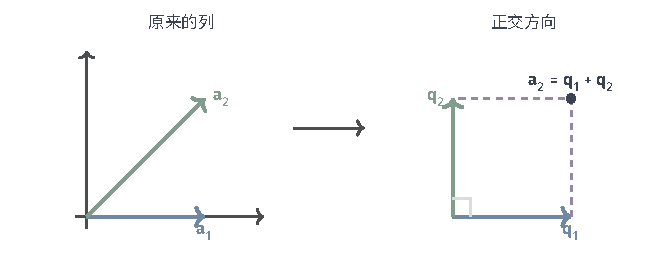
\includegraphics[width=112mm]{figures/00-shared/mathematical-preliminaries-upper/02-linear-spaces/tikz/comprehension-additions/linear-qr-columns.pdf}
  \caption{QR分解把列的方向和组合系数分开。取$\bm a_1=(1,0)^\top$、$\bm a_2=(1,1)^\top$，
  正交化得到$\bm q_1=(1,0)^\top$、$\bm q_2=(0,1)^\top$，并有$\bm a_1=\bm q_1$、
  $\bm a_2=\bm q_1+\bm q_2$，故$\bm R=\left[\begin{smallmatrix}1&1\\0&1\end{smallmatrix}\right]$。
  虚线补出第二列的分量。}
  \label{fig:vol1-add-linear-qr-columns}
\end{figure}

这一分解的用处在于，涉及列空间的计算可以改在标准正交的$\bm Q$上进行，坐标由内积直接读出，不必再解Gram方程。第~\ref{chap:linear-solution-selection}章与第~\ref{chap:direct-linear-solvers}章解方程与最小二乘问题时就是这样使用它的。

\subsubsection{列相关时的处理}

定理~\ref{thm:ls-gram-schmidt}要求各列线性无关。若不满足，某一步会出现$\bm u_j=\bm0$。由正交分解，这恰好说明$\bm a_j$已在前面方向张成的空间中，没有带来新方向。这时不能对零向量归一化，应跳过这一列，只在$\bm R$中记下它的系数$\langle\bm a_j,\bm q_i\rangle$。跳过它不影响后续各列，因为张成的空间没有变。

全部处理完以后，留下的$\bm q$的个数等于列空间的维数$r=\operatorname{rank}\bm A$，仍有$\bm A=\bm Q\bm R$。其中$\bm Q\in\mathbb R^{m\times r}$的列是列空间的标准正交基；$\bm R\in\mathbb R^{r\times d}$各行从左到右第一个非零元的位置逐行右移。$r<d$时$\bm R$不是方阵，不能求逆。下面是最小的例子。
\begin{example}[列相关时跳过零余量]
\label{ex:ls-qr-dependent-columns}
设$\bm A=[\bm a_1\ \bm a_2]$，其中$\bm a_1=(1,0)^\top$、$\bm a_2=(2,0)^\top$，第二列是第一列的两倍。$\bm a_1$已是单位向量，$\bm q_1=\bm a_1$。处理第二列时，$\langle\bm a_2,\bm q_1\rangle=2$，扣除后
\[
 \bm u_2=\bm a_2-2\bm q_1=\bm0,
\]
第二列没有带来新方向。于是跳过$\bm a_2$，只在$\bm R$中记下系数$2$，得到$r=1$，
\[
\begin{gathered}
\bm Q=\begin{bmatrix}1\\0\end{bmatrix},\\
\bm R=\begin{bmatrix}1&2\end{bmatrix},\\
\bm Q\bm R=\begin{bmatrix}1&2\\0&0\end{bmatrix}=\bm A .
\end{gathered}
\]
乘回去仍得到$\bm A$，说明跳过的列并没有丢失信息，它的系数保存在$\bm R$中。

列空间是$x$轴，$\bm Q$的唯一一列构成它的标准正交基，留下的列数$1$正是$\operatorname{rank}\bm A$；$\bm R$是$1\times2$矩阵，不能求逆。
\end{example}
于是在精确算术下，同一过程也给出列空间的一组标准正交基与矩阵的秩。有限精度下，扣除后的余量很少恰好为零；怎样判断它“算作零”，以及怎样改写扣除顺序以减少正交性的损失，属于数值计算问题，在第~\ref{sec:ls-numerical-sensitivity}节讨论。

\subsection{正交投影}
\label{sec:ls-orthogonal-projection}

标准正交基使子空间中的分量可以逐个读出。把这些分量合在一起，就得到正交投影。本小节证明它是子空间中离原向量最近的点，再把它写成矩阵，并给出判断一个矩阵是否为正交投影的方法。

\paragraph{向子空间的正交分解}
若$\bm q_1,\ldots,\bm q_r$是子空间$U$的标准正交基，引理~\ref{lem:ls-orthogonal-decomposition}中的Gram矩阵是单位矩阵，Gram方程直接给出$\bm a=(\langle\bm q_i,\bm x\rangle)_i$。于是分解可以直接写出：
\begin{equation}
 \bm x=\underbrace{\sum_{j=1}^r\langle\bm x,\bm q_j\rangle\bm q_j}_{\bm u\in U}+\underbrace{\Bigl(\bm x-\sum_{j=1}^r\langle\bm x,\bm q_j\rangle\bm q_j\Bigr)}_{\bm r\in U^\perp}.
 \label{eq:ls-orthonormal-projection}
\end{equation}
$\bm u$称为$\bm x$在$U$上的正交投影。$\bm u$与$\bm r$正交，由勾股定理，
\[
 \lVert\bm x\rVert^2=\lVert\bm u\rVert^2+\lVert\bm r\rVert^2\geq\sum_{j=1}^r\langle\bm x,\bm q_j\rangle^2.
\]
即沿一部分标准正交方向读出的系数，其平方和不超过总长度的平方；等号恰在$\bm x\in U$时成立。

$\bm u$正是子空间中离$\bm x$最近的点。
\begin{theorem}[正交投影是最近点]
\label{thm:ls-orthogonal-projection-nearest}
设$U$是内积空间$V$的有限维子空间，$\bm x\in V$，$\bm u$是$\bm x$在$U$上的正交投影。对任意$\bm v\in U$，
\[
 \lVert\bm x-\bm v\rVert^2=\lVert\bm x-\bm u\rVert^2+\lVert\bm u-\bm v\rVert^2,
\]
因此$\lVert\bm x-\bm v\rVert\geq\lVert\bm x-\bm u\rVert$，等号当且仅当$\bm v=\bm u$。也就是说，$\bm u$是$U$中唯一离$\bm x$最近的点。
\end{theorem}
\begin{proof}
$\bm x-\bm v=(\bm x-\bm u)+(\bm u-\bm v)$的两项分别属于$U^\perp$和$U$，彼此正交，由勾股定理即得等式。右端第二项非负，并且只在$\bm v=\bm u$时为零。
\end{proof}
基不是标准正交时，同样可以先解Gram方程求出投影；实际求解时不必显式形成逆矩阵。

最近点的唯一性来自内积确定的正交分解。第~\ref{sec:ls-quotient-norms}节已经证明一般范数下最近点存在，示例~\ref{ex:ls-linf-nonunique-nearest}却在$\ell_\infty$范数下给出了无穷多个最近点；同一个点在欧氏范数下的最近点只有原点，因为
\[
 \lVert\bm y-(t,0)^\top\rVert_2^2=t^2+1
\]
只在$t=0$时取最小值。

下面用标准正交基重算前面的正交分解。
\begin{example}[用标准正交基重算正交分解]
\label{ex:ls-orthonormal-projection-line}
回到示例~\ref{ex:ls-orthogonal-decomposition-line}的$\bm y=(1,1.1,0.9)^\top$与直线$U$，这次先把方向向量归一化为$\bm q_1=(1,1,1)^\top/\sqrt3$，于是$U=\operatorname{span}\{\bm q_1\}$。投影系数就是一次内积，由它得到投影与余量：
\[
 \begin{gathered}
 \langle\bm y,\bm q_1\rangle=\frac3{\sqrt3}=\sqrt3,\qquad
 \sqrt3\,\bm q_1=(1,1,1)^\top,\\
 \bm y-\sqrt3\,\bm q_1=(0,0.1,-0.1)^\top .
 \end{gathered}
\]
余量与$\bm q_1$正交。

结果与前例相同，但这里不需要解Gram方程：归一化已经把Gram矩阵变成了$1$。由上面的最近点性质，$(1,1,1)^\top$还是直线$U$上离$\bm y$最近的点。
\end{example}

\paragraph{投影矩阵}
\label{sec:ls-projection-matrices}
正交投影随原向量线性变化。记$\bm y$在$U$上的正交投影为$\bm p$。$\bm y_1,\bm y_2$的正交分解相加、数乘后仍是正交分解，由分解的唯一性，投影也随之相加、数乘。所以$\bm y\mapsto\bm p$是一个线性映射，称为到$U$的正交投影。

在欧氏内积下，它可以写成矩阵。设$\bm Q$的列是$U$的标准正交基。按矩阵乘积的列读法，
\[
 \bm p=\sum_j\langle\bm q_j,\bm y\rangle\bm q_j=\bm Q\bm Q^\top\bm y,
\]
所以到$U$的正交投影是
\begin{equation}
\begin{gathered}
\bm P_U=\bm Q\bm Q^\top,\\
\bm P_U^\top=\bm P_U,\\
\bm P_U^2=\bm P_U.
\end{gathered}
\label{eq:linear-algebra-orthogonal-projector}
\end{equation}
两条性质都可以直接验证。由$\bm Q^\top\bm Q=\bm I$，
\[
 \bm P_U^2=\bm Q(\bm Q^\top\bm Q)\bm Q^\top=\bm Q\bm Q^\top=\bm P_U,
\]
即幂等：已经在$U$中的点再投影一次不变。又$(\bm Q\bm Q^\top)^\top=\bm Q\bm Q^\top$，即对称：内积中可以把投影移到另一侧。

此外$\operatorname{range}\bm P_U=\operatorname{range}\bm Q=U$。$\bm Q$不是方阵时，$\bm P_U$通常不是单位矩阵，它只保留$U$中的分量。

\paragraph{正交投影、斜投影与幂等}
拿到一个矩阵，怎样判断它是不是正交投影？幂等性只说明它是某种投影，不说明它给出最近点。一般的幂等矩阵$\bm P$把$\bm y$分成$\bm P\bm y$与$\bm y-\bm P\bm y$两部分，前者在像中，后者在零空间中，因为$\bm P(\bm y-\bm P\bm y)=\bm P\bm y-\bm P^2\bm y=\bm0$。但两部分不必正交。这种映射称为\term{斜投影}（oblique projection）。

\begin{example}[反例：幂等而不对称的投影]
\label{ex:ls-oblique-projection}
取
\[
 \bm P=\begin{bmatrix}1&-1\\0&0\end{bmatrix}.
\]
直接相乘得$\bm P^2=\bm P$，所以它幂等；它把$(y_1,y_2)^\top$送到$x$轴上的$(y_1-y_2,0)^\top$。

残差$\bm y-\bm P\bm y=(y_2,y_2)^\top$与$x$轴方向$(1,0)^\top$的内积是$y_2$，$y_2\neq0$时不为零，所以$\bm P\bm y$不是$x$轴上离$\bm y$最近的点。这个$\bm P$也不对称：$\bm P^\top\neq\bm P$。
\end{example}

对称性正是正交的条件。若$\bm P$幂等且对称，对任意$\bm y,\bm z$有
\[
 (\bm y-\bm P\bm y)^\top\bm P\bm z=\bm y^\top(\bm P-\bm P^\top\bm P)\bm z=\bm y^\top(\bm P-\bm P^2)\bm z=0,
\]
即残差与整个像正交。于是$\bm y=\bm P\bm y+(\bm y-\bm P\bm y)$是$\bm y$关于像空间的正交分解，由分解的唯一性，$\bm P$就是到其像的正交投影。

所以判别分两步：先验幂等，判断是不是投影；再验对称，判断是不是正交投影。
